\section{Ecossistema de software acadêmico de análise estática} \label{analise-estatica}

Ao falarmos sobre ecossistema de software acadêmico estamos nos referindo a
qualquer software, de qualquer domínio de aplicação, que tenha sido utilizado
ou produzido durante trabalhos de pesquisa com intuito de publicação na
literatura acadêmica.

O ecossistema de software acadêmico de análise estática é um recorte deste
conjunto, a princípio, com as mesmas características, atores e modelo de
funcionamento, mas logicamente podendo apresentar particularidades trazidas
pela natureza do domínio de análise estática e suas ferramentas, soluções e
algoritmos.

\subsection{Análise estática}

A análise estática de código-fonte é o primeiro passo para coletar informações
necessárias em diversas atividades de verificação, medição e melhoria da
qualidade de produtos de software \cite{cruz2009code, kirkov2010source}. Ela é
realizada com base no código-fonte de um programa ou sistema de software, e a
partir daí descobre problemas e propriedades de sua qualidade estrutural
\cite{chess2007secure}.

Ferramentas de análise estática estão disponíveis há décadas, em especial,
para programadores. A ferramenta Lint \cite{johnson1978lint}, considerada uma das
primeiras ferramentas de análise estática \cite{gosain2015static}, foi criada para
examinar programas escritos em linguagem C e aplicar regras de tipagem mais
estritas do que as regras dos próprios compiladores da linguagem.

Análise estática de código-fonte tem como objetivo prover
informações acerca de um programa a partir do seu código-fonte sem
necessidade de execução, e sem requerer qualquer outro artefato do programa
além do próprio código.

É um ramo que possui muitas das suas abordagens em comum com os estudos da
área de análise de programas ({\it program analysis}), especialmente na área de
compiladores, onde atua especialmente nas primeiras etapas do processo de compilação.

A análise estática de código-fonte é considerada uma atividade meio com
objetivo de suportar uma variedade de tarefas comuns da Engenharia de
Software; muitas dessas tarefas são substancialmente úteis em atividades de
manutenção, como por exemplo,
análise de performance,
compreensão de programas,
desenvolvimento baseado em modelos,
detecção de clones,
evolução de software,
garantia de qualidade,
localizaçao de falhas,
manutenção de software,
recuperação arquitetural e
testes \cite{binkley2007source}.

Seja em qual atividade for, a análise estática possui importância
significativa, pois ao ser capaz de extrair informações diretamente do
código-fonte de um programa, pode auxiliar a responder perguntas necessárias
para as diversas atividades de desenvolvimento e evolução de software. Essa
importância se torna ainda mais aparente diante da ``lei'' da tendência para
execução que indica que todos os tipos de notação têm a tendência de se tornar
executáveis.  Cada nova notação, seja de baixo nível (e, portanto, já
código-fonte) ou de alto nível (podendo escapar do nível de código) irá em
última análise se tornar código-fonte \cite{harman2010why}.

A análise de programas trata, de modo geral, da descoberta de problemas e
fatos sobre programas. Tal análise pode ser realizada sem a necessidade de executar o
programa (análise estática) ou com informações provenientes de sua execução
(análise dinâmica).

A ideia de que programas de computador podem ser utilizados para analisar
código-fonte de outros programas tem uma história de mais de 40 anos.  O
programa {\it PFORT Verifier} \cite{ryder1974pfort} foi projetado para localizar potenciais
problemas na portabilidade de código Fortran; em função da diversidade de
dialetos de Fortran, uma compilação sem erros não indicava que o programa
estava correto segundo os padrões da linguagem \cite{wichmann1995industrial}.

Desde então, ferramentas de análise estática de código-fonte têm surgido para
os mais diversos fins -- muitas delas a partir das pesquisas e
desenvolvimentos da área de compiladores.  O {\it parser} utilizado nessas
ferramentas têm funcionalidades análogas aos analisadores usados em
compiladores \cite{anderson2008the}.

O uso de tais ferramentas tem se tornado mais comum no ciclo de desenvolvimento de
software, sendo aplicadas em atividades distintas.
O campo de aplicação destas ferramentas é bastante variado, cobrindo diferentes
objetivos.

\subsection{Software de análise estática}

A variedade de aplicação e a constante evolução da área de análise estática, 
tanto na indústria quando na academia, resulta em  estudos teóricos e práticos, novas ferramentas, modelos e
algoritmos de análise estática. Ferramentas de análise estática têm sido
continuamente desenvolvidas e seu uso se tornado comum no ciclo de desenvolvimento de
software.

Mas apesar da rápida e constante evolução da área, ainda há carência de estudos
avaliando estas ferramentas \cite{li2010comparative}. Mesmo com os avanços e com
ferramentas de sucesso, o desenvolvimento de análise estática ainda é conhecido
por ser um processo doloroso \cite{toman2017taming}.

A eficiência, confiabilidade e precisão dessas ferramentas têm sido avaliadas e
alguns estudos mostram inconsistência entre ferramentas diferentes.  Um desses
estudos comparou duas ferramentas de análise estática para cálculo de métricas
e revelou significantes evidências sobre a inconsistencia entre valores de
métricas, mostrando grande diferença entre os valores e discutindo quais
problemas e questões levam a tais diferenças \cite{alemerien2013experimental}.

Análise estática é a técnica mais amplamente utilizada para análise
automatizada de programas devido a sua eficiência, boa cobertura e automação.
Estudos mostram que analise estática tem grande adoção em projetos de software
livre \cite{beller2016analyzing}.
Entretanto, técnicas de análise estática amplamente adotadas na comunidade de software,
por exemplo, para localização de bugs e verificação de programas 
ainda sofrem um alto índice de falso-positivos \cite{gosain2015static}.

Apesar da ampla adoção de ferramentas de análise estática em estudos
acadêmicos e da crescente atenção que as técnicas de análise estática de código tem
recebido em pesquisas, nota-se ainda uma enorme distância entre a atenção dada na academia e sua adoção na indústria,
identificando um {\it gap} entre estes dois contextos \cite{ilyas2016static}.

\subsection{Software acadêmico de análise estática}

Na Ciência da Computação, particularmente na Engenharia de Software, tem-se
notado um aumento constante no número de novos projetos de software acadêmico \cite{allen2017engineering},
especialmente em estudos de análise estática, 
uma área com uma longa e respeitável tradição em
pesquisas sobre a criação de novas ferramentas, métodos e algoritmos.

O software acadêmico de análise estática e o seu ecossistema, ao estar inserido
no sistema acadêmico e intimamente relacionado à economia de reputação
científica, sofre as consequências da competição que permeia este modelo, e o
seu uso invariavelmente deixa de gerar {\it feedback} positivo de volta ao seu ecossistema,
conforme Figura \ref{scientific-reputation-diagram}, onde se apresenta o
relacionamento entre a prática e a pesquisa de software acadêmico.

\begin{figure}[h]
  \center
  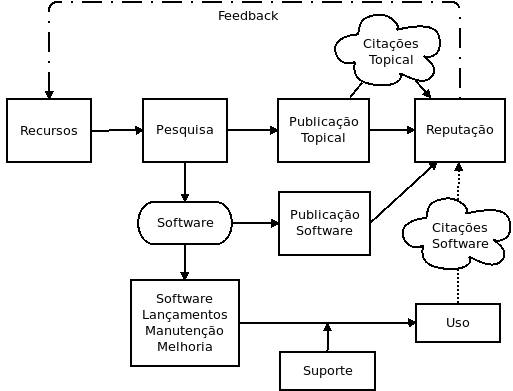
\includegraphics[scale=0.35]{imagens/scientific-reputation-diagram.png}
  \caption{Uma visão dos incentivos de reputação num contexto misto entre Ciência e práticas de software acadêmico \cite{howison2011scientific}}
  \label{scientific-reputation-diagram}
\end{figure}

A Figura \ref{scientific-reputation-diagram} apresenta a situação enfrentada
por muitos cientistas que distribuem software com intenção de ser utilizado por
outros, há incertezas sobre o recebimento de citações para o software
através do seu uso, esta incerteza é indicada na figura através da ligação pontilhada entre o uso do
software e a reputação obtida através de citações. Diferentemente da
publicação científica regular ({\it Publicação topical}), a publicação do software
raramente é útil por si mesma; geralmente é o software que é útil para outros
cientistas, no entanto, nem todos os usuários de software acadêmico vêem como
requisito citar o software, a nem todos os projetos de software acadêmico
indicam uma forma conveniente de como deve ser citado.

Diferentemente de outras tecnologias, software pode ser copiado e distribuído
essencialmente sem custo, abrindo portas sem precedentes para
compartilhamento e inovação colaborativa \cite{howison2011scientific}. No
entanto, por estar de alguma forma conectado ao contexto de competição da economia de
reputação científica, como no mecanismo de crédito acadêmico aos artigos e publicações,
pode ser potencialmente problemático para a colaboração e manutenção
\cite{howison2011scientific}.

Este cenário, além de desacelerar o progresso geral da Ciência gerando
retrabalho, faz surgir questionamentos sobre as conclusões dessas pesquisas,
especialmente quando grande parte dos pesquisadores não sabem o quão confiável
seus projetos de software são. Criando assim, um contexto em que muitos estudos
em Engenharia de Software sofrem de dificuldades de repetição
\cite{tang2016worthiness}, além de ocasionar problemas específicos relacionados a
manutenibilidade e sustentabilidade técnica do software acadêmico.
